\documentclass{article}
\usepackage{graphicx}
\usepackage{authblk}
\usepackage{amsmath}


\begin{document}


\title{THEORETICAL NEUROSCIENCE II \\ EXERCISE 01-02}
\date{21 Apr. 2013}
\author[1]{Yunus Emre Demiray, Taygun Caglayan, \c{S}eyma Bayrak\thanks{seyma.bayrak@st.ovgu.de}}
\affil[1]{\footnotesize  Otto von Guericke University of Magdeburg}
\maketitle

\newpage

\section{Two Dimensional Linear System}

\begin{equation}
 \frac{dE}{dt}=\frac{1}{\tau}(E-\alpha I +K)
\end{equation}

\begin{equation}
  \frac{dI}{dt}=\frac{1}{\tau}(-I+\beta E-4K)
\end{equation}

\begin{itemize}
 \item How does the map of state space of activity E and I look like, if the both equations are solved numerically with the initial values $E_0=3$ and $I_0=3$? Try this out for two different K values that of 0 and 4. 
\end{itemize}

\begin{center}
 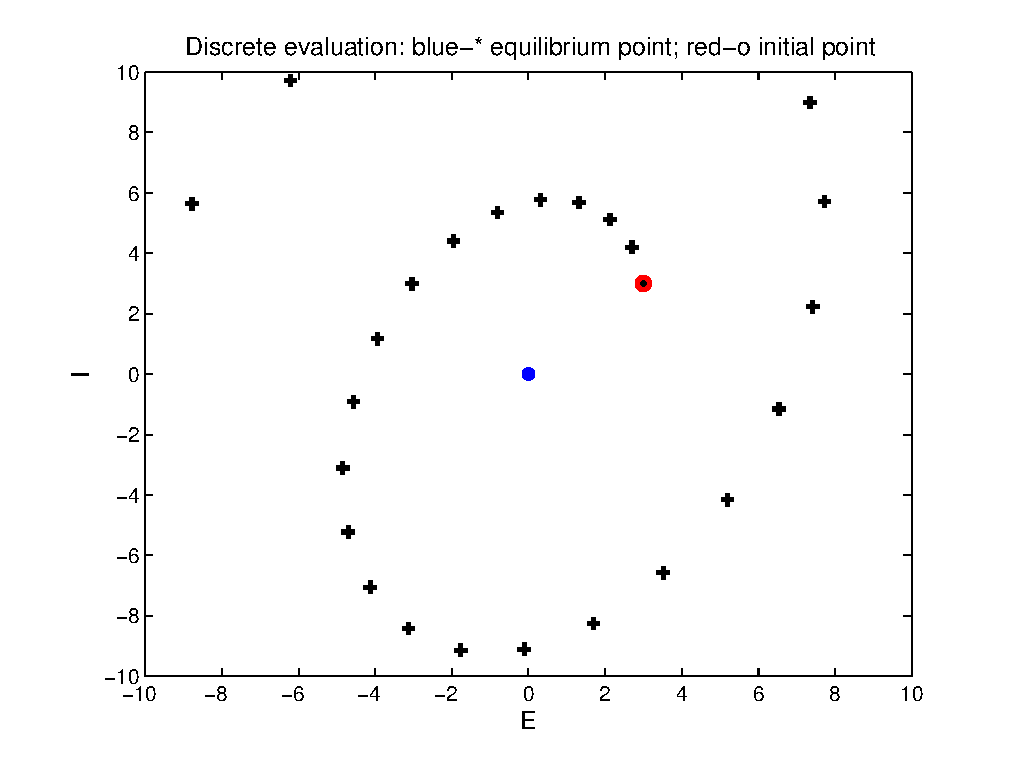
\includegraphics[width=\textwidth]{nonlinear1.eps}
 % q7.eps: 0x0 pixel, 300dpi, 0.00x0.00 cm, bb=  -86   231   682   610
\begin{footnotesize}Figure 1, K=0. Discrete Evaluation of E and I independently from time, red circle represents the initial points $E_0$ and $I_0$ this is a map of state space\end{footnotesize}
\end{center}

\begin{center}
 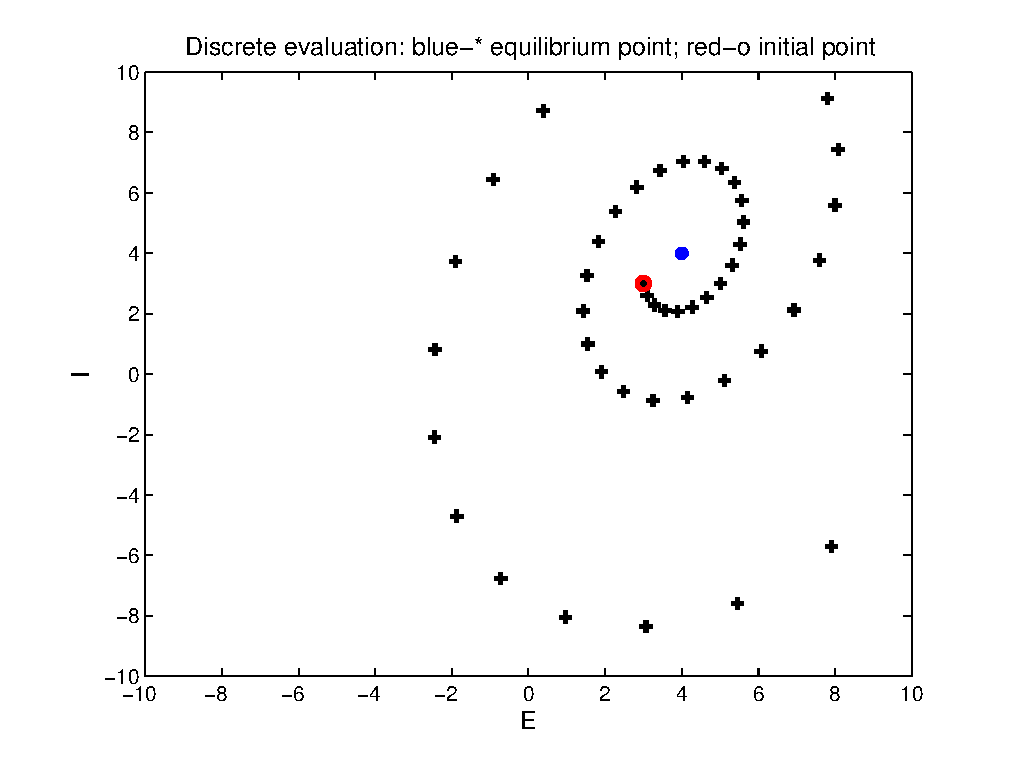
\includegraphics[width=\textwidth]{nonlinear2.eps}
 % q7.eps: 0x0 pixel, 300dpi, 0.00x0.00 cm, bb=  -86   231   682   610
\begin{footnotesize}Figure 2, K=4. Discrete Evaluation of E and I independently from time, red circle represents the initial points $E_0$ and $I_0$\end{footnotesize}
\end{center}


\begin{itemize}
 \item Deriving the isocline and  dynamic flowfield equations:
\end{itemize}

Isocline equations are derived by setting $ \frac{dE}{dt}=0 $ and $ \frac{dI}{dt} $ as the following, note that the given values are inserted for the parameters such that $\tau=10$, $\alpha=2$ and $\beta=5$

\begin{equation*}
  \frac{dE}{dt}=0\longrightarrow \frac{1}{\tau}(E-2I+K)=0\longrightarrow I_1=\frac{E+K}{2}
\end{equation*}

\begin{equation*}
  \frac{dI}{dt}=0\longrightarrow \frac{1}{\tau}(-I+5E-4K)=0\longrightarrow I_2=5E-4K
\end{equation*}

Isoclines are easy to calculate in case the E values are already known, the K value is already assigned to either 0 or 4. Let us choose a range of E values such that $E=-10:0.25:10$. For each value of E, $I_1$ and $I_2$ can be computed and saved inside a matrix, the general row-structure of the isocline matrix is given below.

\begin{equation*}
  isocline(i,:)=[E \;\;\;\; \frac{1}{2}(E+K) \;\;\;\; 5E-4K]
\end{equation*}

Dynamic flow field considers many different initial points for both of $E_0$ and $I_0$, e.g. $-10\leq E_0 \leq 10$ and $-10\leq I_0 \leq 10$. Each time the corresponding $dE$ and $dI$ values are calculated and plotted. The general row-structure of the flowfield matrix is shown below.

\begin{equation*}
  flowfield(i,:)=[E \;\;\;\; I \;\;\;\; \dfrac{1}{\tau}(E-2 I+K)\;\;\;\; \frac{1}{\tau}(-I+5 E-4K)]
\end{equation*}
  
The flowfield for the two different isoclines are as the following.

\begin{equation*}
  flowfield-I_1(i,:)=[E \;\;\;\; I_1 \;\;\;\;   \dfrac{1}{\tau}(E-2I_1+K)\;\;\;\; \frac{1}{\tau}(-I_1+5E-4K)]
\end{equation*}

\begin{equation*}
  =[E \;\;\;\; \frac{1}{2}(E+K) \;\;\;\;   \dfrac{1}{\tau}(E-2(\frac{1}{2}(E+K))+K)\;\;\;\; \frac{1}{\tau}(-(\frac{1}{2}(E+K))+5E-4K)]
\end{equation*}

\begin{equation*}
  =[E \;\;\;\; \frac{1}{2}(E+K) \;\;\;\;0\;\;\;\; \frac{1}{\tau}(\frac{9}{2}(E-K))]
\end{equation*}

\begin{equation*}
  flowfield-I_2(i,:)=[E \;\;\;\; I_2 \;\;\;\;   \dfrac{1}{\tau}(E-2I_2+K)\;\;\;\; \frac{1}{\tau}(-I_2+5E-4K)]
\end{equation*}

\begin{equation*}
  =[E \;\;\;\; (5E-4K) \;\;\;\;   \dfrac{1}{\tau}(E-2(5E-4K)+K)\;\;\;\; \frac{1}{\tau}(-(5E-4K)+5E-4K)]
\end{equation*}

\begin{equation*}
  =[E \;\;\;\; (5E-4K) \;\;\;\;   \dfrac{1}{\tau}(9(K-E))\;\;\;\; 0]
\end{equation*}

\begin{itemize}
 \item Defining the intersection of two isoclines and therefore the equilibrium point $P_{eq}$:
\end{itemize}

The intersection of $I_1$ and $I_2$ is the point where they are equal.

\begin{equation*}
 I_1=I_2 \longrightarrow \frac{1}{2}(E'+K)=5E'-4K \longrightarrow E'=K
\end{equation*}

\begin{equation}
 P_{eq}=(E,E')=(K,K)
\end{equation}

Let us plot dynamic flowfields, isoclines and the $P_{eq}$ on the same graph for two different K values. 
\begin{center}
 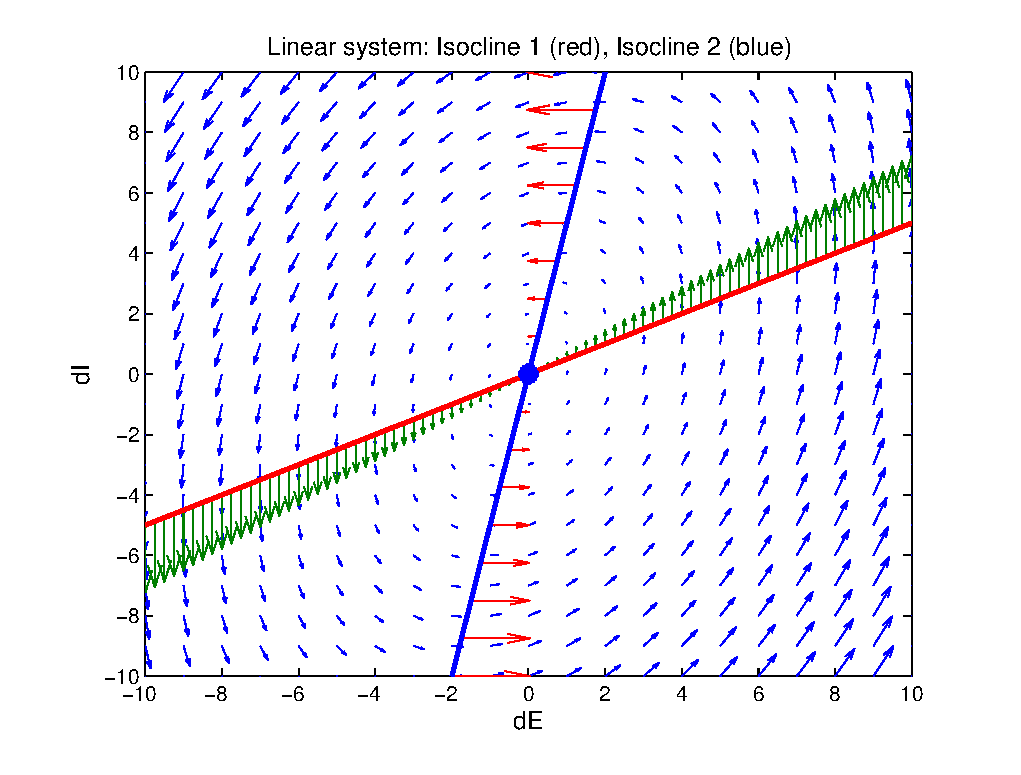
\includegraphics[width=\textwidth, height=8cm]{nonlinear3.eps}
 % q7.eps: 0x0 pixel, 300dpi, 0.00x0.00 cm, bb=  -86   231   682   610
\begin{footnotesize}Figure 3, K=0. The small blue arrows indicate the dynamic flowfields, the red line represents isocline $E$ vs $I_1$ and the blue one that of $E$ vs $I_2$. The blue circle is $P_{eq}=(0,0)$ \end{footnotesize}
\end{center}


\begin{center}
 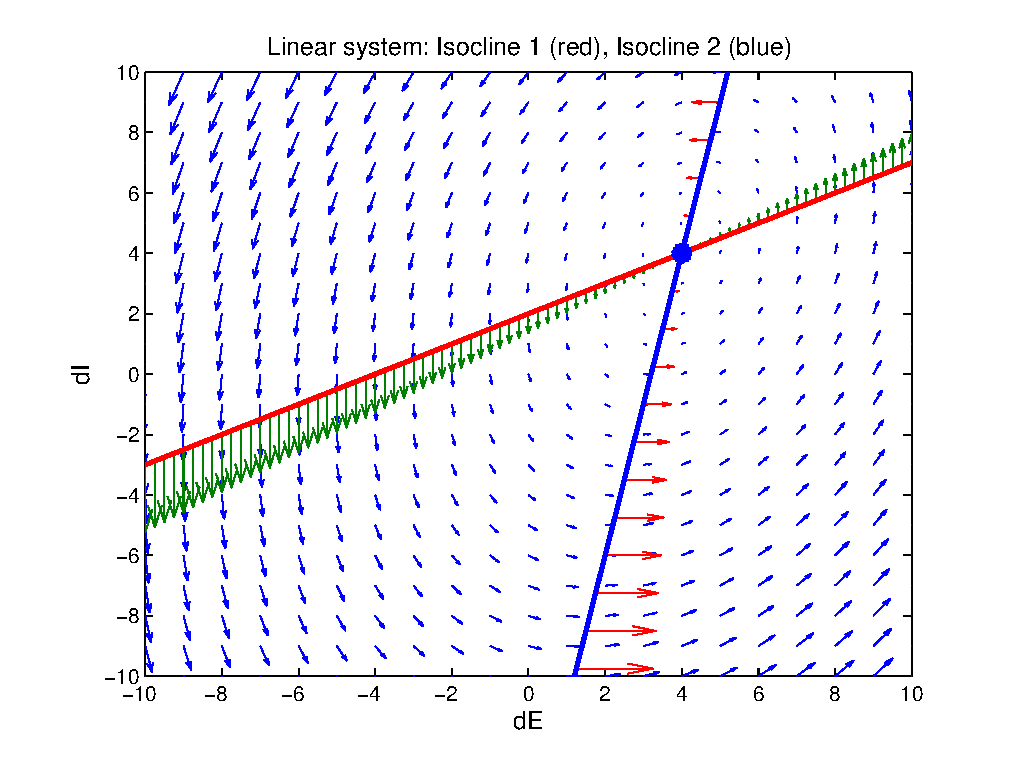
\includegraphics[width=\textwidth, height=8cm]{nonlinear4.eps}
 % q7.eps: 0x0 pixel, 300dpi, 0.00x0.00 cm, bb=  -86   231   682   610
\begin{footnotesize}Figure 4, K=4. The small blue arrows indicate the dynamic flowfields, the red line represents isocline $E$ vs $I_1$ and the blue one that of $E$ vs $I_2$. The blue circle is $P_{eq}=(4,4)$ \end{footnotesize}
\end{center}

\newpage

\begin{itemize}
 \item Define the Jacobian Matrix for each K value as the following, and calculate the eigenvalues of this matrix:
\begin{equation}
F_E\equiv \frac{dE}{dt}, \;\;\;\; F_I\equiv \frac{dI}{dt}, \;\;\;\;            \binom{\frac{\delta F_E}{\delta E} \;\;\; \frac{\delta F_E}{\delta I} }{\frac{\delta F_I}{\delta E} \;\;\; \frac{\delta F_I}{\delta I}}
\end{equation}
\end{itemize}
Let us find out Jacobian Matrix step by step;
\begin{equation*}
 F_E=\frac{1}{\tau}(E-2I+K)\longrightarrow \frac{\delta F_E}{\delta E}=\frac{1}{\tau}, \;\;\;\; \frac{\delta F_E}{\delta I}=\frac{-2}{\tau} 
\end{equation*}

\begin{equation*}
 F_I=\frac{1}{\tau}(-I+5E-4K)\longrightarrow \frac{\delta F_I}{\delta E}=\frac{5}{\tau}, \;\;\;\; \frac{\delta F_I}{\delta I}=\frac{-1}{\tau} 
\end{equation*}
Now insert that $\tau=10$ and write the final version of Jacobian Matrix. 
\begin{equation*}
 \binom{\frac{1}{10} \;\;\;\; \frac{-1}{5}}{\frac{1}{2} \;\;\;\; \frac{-1}{10}}
\end{equation*}
Let us calculate the eigenvalues of that matrix by the help of the eqaution 5.
\begin{equation}
 det(J-\lambda I)=0
\end{equation}

\begin{equation*}
 \binom{\frac{1}{10}-\lambda \;\;\;\; \frac{-1}{5}}{\;\;\;\;\;\;\;\;\; \frac{1}{2}\;\;\;\;\;\;\;\;\;\; \frac{-1}{10}-\lambda\;\;\;\;}=0 \longrightarrow \lambda^{2}+\frac{9}{100}=0
\end{equation*}
The eigenvalues of the Jabobian matrix above are $\lambda_1=0+0.3i$ and $\lambda_2=0-0.3i$. Since the Jacobian Matrix for the linear system is independent of $K$, it is same for both $K=0$ aand $K=4$ values, therefore also the eigenvalues are the same. The complex part of eigenvalues can be ignored, so both eigenvalues can be assumed to be 0, it means that the system is not stable. 

\section{Two-dimensional non-linear system}

\begin{equation}
 \frac{dE}{dt}=\frac{1}{\tau_E}[-E+S(\alpha E-I+K)]
\end{equation}
\begin{equation}
 \frac{dI}{dt}=\frac{1}{\tau_I}[-I+S(\beta E)]
\end{equation}
where $\tau_E=5$, $\tau_I=10$, $\alpha=1.6$, $\beta=1.5$, K is the external input equals to either 0 or 20. 
\begin{equation}
 S(x)=\frac{Mx^2}{\sigma^2+x^2} \;\;\;\;for\;\;\;x\geq0\;\;\;\;or\;\;\;\;S(x)=0\;\;\;\;for\;\;\;x<0
\end{equation}
The function $S$ turns out to be $S(\alpha E-I+K)=\frac{M(\alpha E-I+K)^2}{\sigma^2+(\alpha E-I+K)^2}$ for the equations above (in case $(\alpha E-I+K)\geq0$, otherwise it becomes 0).

\begin{itemize}
 \item How does E vs I look like in state space?
\end{itemize}

Let us choose initial points as $E_0=76.6339$ and $I_0=21.9285$. The numerical integration for the state space - independently from time -gives the following graphs for two different K values.
\begin{center}
 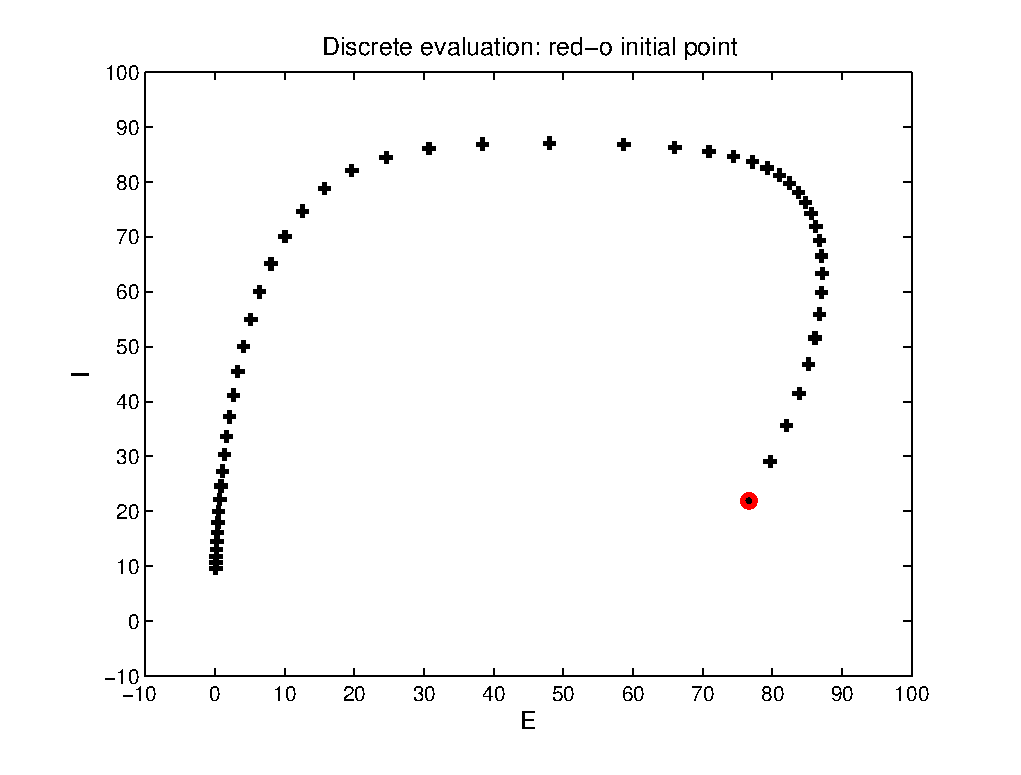
\includegraphics[width=\textwidth, height=7cm]{linear1.eps}
 % q7.eps: 0x0 pixel, 300dpi, 0.00x0.00 cm, bb=  -86   231   682   610
\begin{footnotesize}Figure 5, K=0. State spave map of E vs I, the red circle stands for the initial points $E_0$ and $I_0$\end{footnotesize}
\end{center}


\begin{center}
 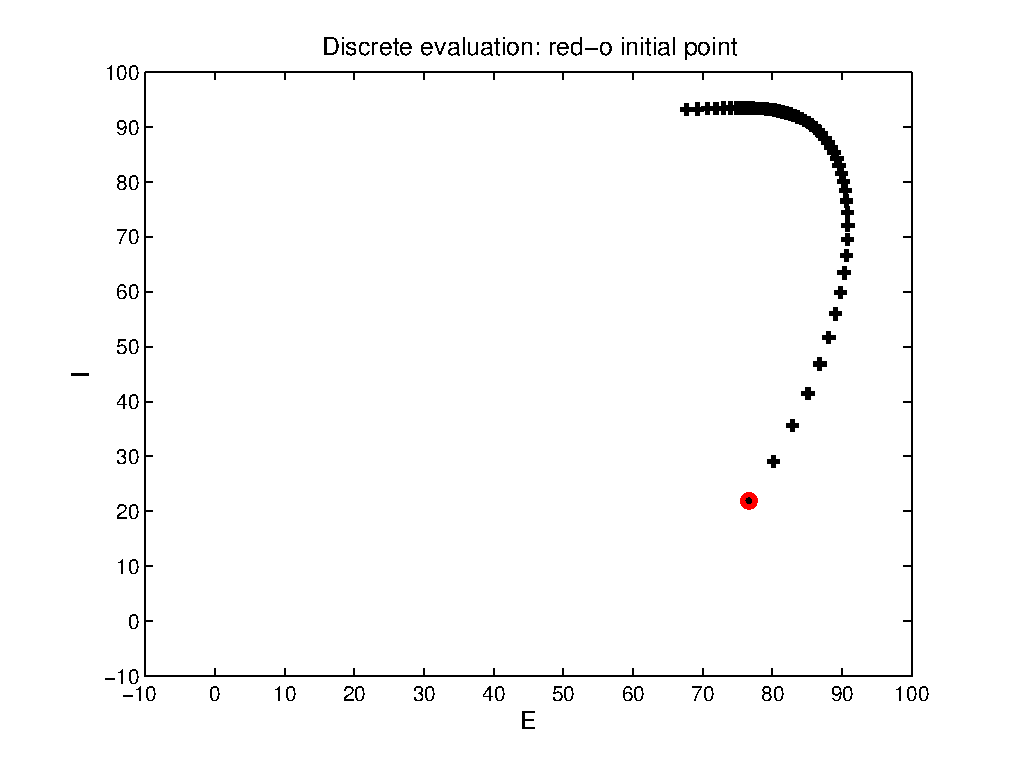
\includegraphics[width=\textwidth, height=7cm]{linear2.eps}
 % q7.eps: 0x0 pixel, 300dpi, 0.00x0.00 cm, bb=  -86   231   682   610
\begin{footnotesize}Figure 6, K=20. State spave map of E vs I, the red circle stands for the initial points $E_0$ and $I_0$.  \end{footnotesize}
\end{center}

\begin{itemize}
 \item Derivation of isoclines of non-linear system:
\end{itemize}

\begin{equation*}
\frac{dI}{dt}=0\longrightarrow -I+S(\beta E)=0\longrightarrow I_1=S(\beta E)\longrightarrow I_1=\frac{M(\beta E)^2}{\sigma^2+(\beta E)^2} 
\end{equation*}

\begin{equation*}
 \frac{dE}{dt}=0\rightarrow -E+S(\alpha E-I+K)=0 \rightarrow
\end{equation*}
\begin{equation*}
I_2=\alpha E+K-\sqrt{\frac{E \alpha^2}{M-E}} \;\;\;\;\; I_3=\alpha E+K+\sqrt{\frac{E \alpha^2}{M-E}}
\end{equation*}

Let us choose E values such that $E=0:1:100$ and fill the isocline matrix up, the general-row represantation of isocline matrix is the following.

\begin{equation*}
 isoclines(i,:)=[E \;\;\;\;I_1\;\;\;\; I_2\;\;\;\; I_3]
\end{equation*}
This matrix will be plotted further as $I_1$, $I_2$ and $I_3$ with respect to E. 

\begin{itemize}
 \item Dynamical Flowfields
\end{itemize}
We assume different values for both E and I such that $E=0:5:100$ and $I=0:5:100$, and then for each E and I values, the corresponding flowfield is computed as the following.
\begin{equation*}
flowfield(i,:)=[E\;\;\;\;I\;\;\;\;dE\;\;\;\;dI]
\end{equation*}
\begin{equation*}
 =[E\;\;\;\;I\;\;\;\; \frac{1}{\tau_E}(-E+S(\alpha E-I+K))\;\;\;\; \frac{1}{\tau_I}(-I+S(\beta E))]
\end{equation*}

The flowfield for the isocline $I_1$:
\begin{equation*}
 flowfield-I_1(i,:)=[E\;\;\;\; I_1\;\;\;\;\frac{1}{\tau_E}(-E+S(\alpha E-I_1+K))\;\;\;\; \frac{1}{\tau_I}(-I_1+S(\beta E)]
\end{equation*}
Now insert $I_1$:
\begin{equation*}
 flowfield-I_1(i,:)=[E \;\;\;\;\;\;\;\;S(\beta E)\;\;\;\;\;\;\;\; \frac{1}{\tau_E}(-E+S(\alpha E - S(\beta E)+K))
\end{equation*}
\begin{equation*}
 \;\;\;\;\;\;\;\;\;\;\;\;\;\;\;\;\;\;\;\;\;\;\;\;\;\;\;\; \frac{1}{\tau_I}(-S(\beta E)+S(\beta E)\;\;\;\;]
\end{equation*}

Similarly, the flowfield for the isocline $I_2$ and $I_3$:
\begin{equation*}
 flowfield-I_2(i,:)=[E\;\;\;\; I_2\;\;\;\;\frac{1}{\tau_E}(-E+S(\alpha E-I_2+K))\;\;\;\; \frac{1}{\tau_I}(-I_2+S(\beta E)]
\end{equation*}
\begin{equation*}
 flowfield-I_3(i,:)=[E\;\;\;\; I_3\;\;\;\;\frac{1}{\tau_E}(-E+S(\alpha E-I_3+K))\;\;\;\; \frac{1}{\tau_I}(-I_3+S(\beta E)]
\end{equation*}
where $I_2$ and $I_3$ can be trivially inserted on MATLAB, as calculated before.
\begin{equation*}
I_2=\alpha E+K-\sqrt{\frac{E\sigma^2}{M-E}} \;\;\;\;\; I_3=\alpha E+K+\sqrt{\frac{E\sigma^2}{M-E}}
\end{equation*}

\begin{itemize}
 \item Intersection points of the isoclines:
\end{itemize}

Intersection points are defined as the following;
\begin{equation*}
 I_1=I_2\longrightarrow \frac{M(\beta E)^2}{\sigma^2+(\beta E)^2}=\alpha E+K-\sqrt{\frac{E \alpha^2}{M-E}}
\end{equation*}
and
\begin{equation*}
 I_1=I_3\longrightarrow \frac{M(\beta E)^2}{\sigma^2+(\beta E)^2}=\alpha E+K+\sqrt{\frac{E \alpha^2}{M-E}}
\end{equation*}
The MATLAB command \textit{fsolve} solve the both equations for $E$. For K=0, there are three intersection points between $I_1$ and $I_3$, however, there is no intersection between $I_1$ and $I_2$. Equilibrium points for K=0 are given below.

\begin{equation*}
P_{eq1}=(0,\;\;0) \;\;\;\;\;\;\;\; P_{eq2}=(15.6339,\;\;37.9285) \;\;\;\;\;\;\;\;P_{eq3}=(32.1596,\;\; 72.1106) 
\end{equation*}

 For K=20, there is only one intersection point between $I_1$ and $I_2$, however, there is no intersection between $I_1$ and $I_3$. Equilibrium point for K=20 is given below.

 \begin{equation*}
  P_{eq}=(12.7664,\;\;28.9496)
 \end{equation*}


\begin{itemize}
 \item Plot the isoclines and dynamical flowfields for two different K points:
\end{itemize}

\begin{center}
 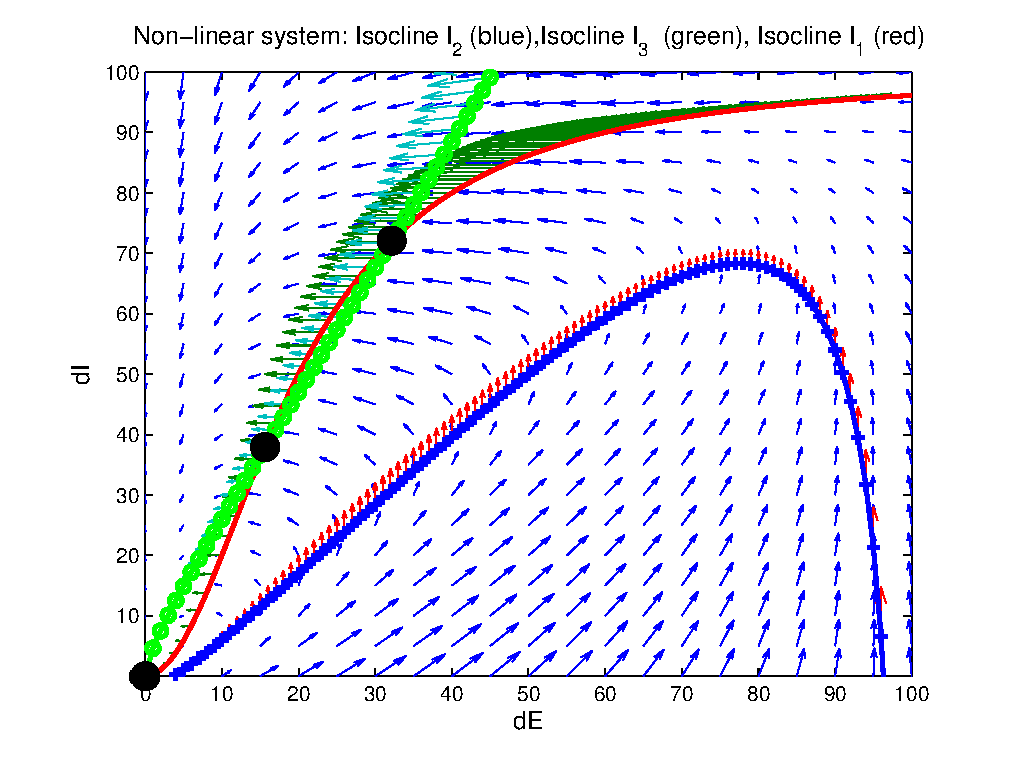
\includegraphics[width=\textwidth, height=8cm]{linear3.eps}
 % q7.eps: 0x0 pixel, 300dpi, 0.00x0.00 cm, bb=  -86   231   682   610
\begin{footnotesize}Figure 7, K=0. Isoclines and flowfields of non-linear equations. Large-dark circles indicate the three intersection points between isoclines $I_3$ and $I_1$ : $P_{eq1}$, $P_{eq2}$ and $P_{eq3}$. \end{footnotesize}
\end{center}
\begin{center}
 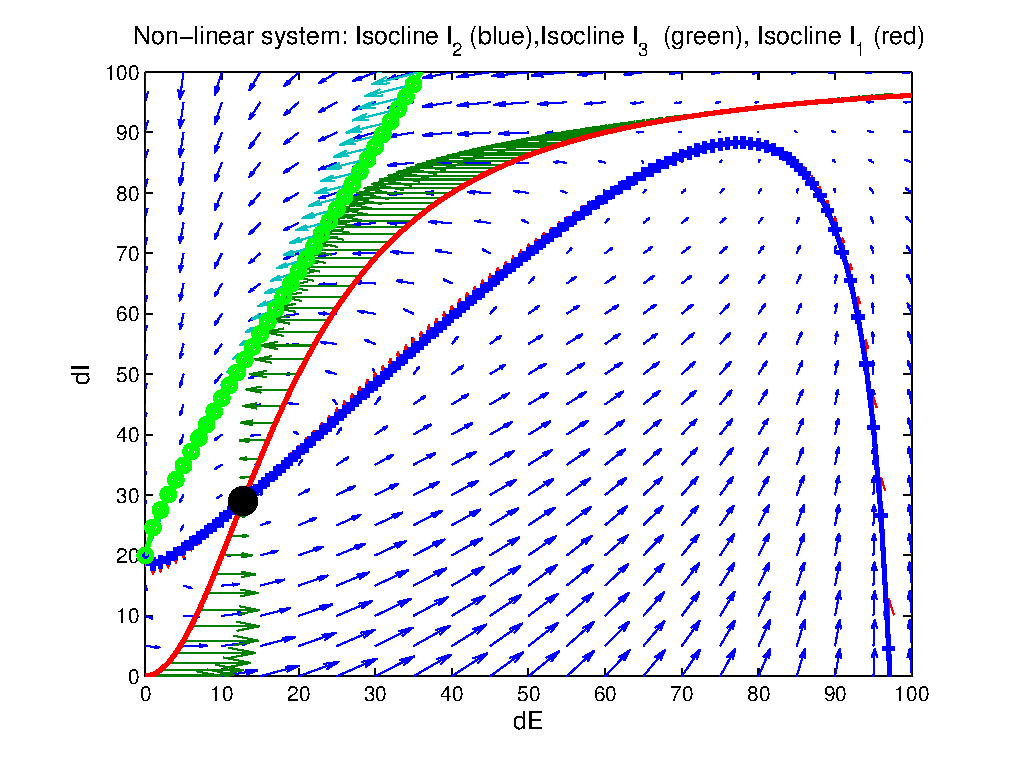
\includegraphics[width=\textwidth, height=8cm]{linear4.eps}
 % q7.eps: 0x0 pixel, 300dpi, 0.00x0.00 cm, bb=  -86   231   682   610
\begin{footnotesize}Figure 8, K=20. Isoclines and flowfields. Large-dark circle represents the intersection point between $I_1$ and $I_2$: $P_{eq}=(12.7664,\;\;28.9496)$ \end{footnotesize}
\end{center}

\begin{itemize}
 \item Jacobian Matrix  for the non-linear system
\end{itemize}
The Jacobian Matrix is derived as it was done in the first section. 
\begin{equation*}
 F_E=\frac{dE}{dt}=\frac{1}{\tau_E}[-E+S(\alpha E-I+K)] 
\end{equation*}

\begin{equation*}
 F_I=\frac{dI}{dt}=\frac{1}{\tau_I}[-I+S(\beta E)]
\end{equation*}

\begin{equation*}
\frac{\delta F_E}{\delta E}=\frac{d}{dE}(\frac{1}{\tau_E}(-E+S(\alpha E-I+K))=\frac{d}{dE}(\frac{1}{\tau_E}(-E+(\frac{M(\alpha E-I+K)^2}{\sigma^2 + (\alpha E-I+K)^2})))
\end{equation*}
\begin{equation*}
 =\frac{1}{\tau_E}[-1+\frac{2M\alpha (\alpha E -I+K)\sigma^2}{(\sigma^2+(\alpha E -I+K)^2)^2}]
\end{equation*}

\begin{equation*}
 \frac{\delta F_E}{\delta I}=\frac{d}{dI}(\frac{1}{\tau_E}[-E+S(\alpha E-I+K)])=\frac{d}{dI}(\frac{1}{\tau_E}(-E+(\frac{M(\alpha E-I+K)^2}{\sigma^2 + (\alpha E-I+K)^2})))
\end{equation*}
 \begin{equation*}
  =\frac{1}{\tau_E}[\frac{-2M(\alpha E-I+K)\sigma^2}{(\sigma^2 + (\alpha E-I+K)^2)^2}]
 \end{equation*}


\begin{equation*}
 \frac{\delta F_I}{\delta E}=\frac{d}{dE}(\frac{1}{\tau_I}[-I+S(\beta E)])=\frac{d}{dE}(\frac{1}{\tau_I}[-I+\frac{M(\beta E)^2}{\sigma^2 + (\beta E)^2}])
\end{equation*}
\begin{equation*}
 =\frac{1}{\tau_I}[\frac{2ME\beta^2 \sigma^2}{(\sigma^2 + (\beta E)^2)^2}]
\end{equation*}



\begin{equation*}
 \frac{\delta F_I}{\delta I}=\frac{d}{dI}(\frac{1}{\tau_I}[-I+\frac{M(\beta E)^2}{\sigma^2 + (\beta E)^2}])=\frac{-1}{\tau_I}
\end{equation*}


\textbf{}
\begin{large}\[
 J=
\left ( \begin{array}{cc}
\frac{1}{\tau_E}[-1+\frac{2M\alpha (\alpha E -I+K)\sigma^2}{(\sigma^2+(\alpha E -I+K)^2)^2}] & \frac{1}{\tau_E}[\frac{-2M(\alpha E-I+K)\sigma^2}{(\sigma^2 + (\alpha E-I+K)^2)^2}] \\
\frac{1}{\tau_I}[\frac{2ME\beta^2 \sigma^2}{(\sigma^2 + (\beta E)^2)^2}] & \frac{-1}{\tau_I} 
\end{array} \right )
\]\end{large}


\begin{itemize}
 \item Fill out Jacobian Matrix with the help of intersection points and find eigenvalues of it, determine whether the system is stable or not:
\end{itemize}

Note that the parameters are the following; $1/\tau_E=5$, $1/\tau_I=1.6$, $\beta=1.5$, $M=100$ and finally $\sigma=30$. The value $K$ is either 0 or 20.
We need to analyze the system at each intersection point separately.\\

For $K=0$ and $P_{eq1}=(0,0)$, the Jacobian matrix turns out to be the following below (that means $E=0$ and $I=0$ ):

\textbf{}
\begin{large}\[
 J_1=
\left ( \begin{array}{cc}
-0.2 & 0 \\
0 & -0.1
\end{array} \right )
\]\end{large}

The eigenvalues of the matrix above are $\lambda_1=-0.2$ and $\lambda_2=-0.1$. Since the both eigenvalues are below zero, the system is said to be stable at $P_{eq1}=(0,0)$.\\

For $K=0$ and $P_{eq2}=(15.6339, 37.9285)$, the Jacobiam Matrix is the following:

\textbf{}
\begin{large}\[
 J_2=
\left ( \begin{array}{cc}
   -0.8536  &  0.4085 \\
    0.3012  & -0.1000
\end{array} \right )
\]\end{large}

The eigenvalues of the matrix above are $\lambda_1=-0.9916$ and $\lambda_2=0.0380$. Since the both eigenvalues are not below zero, the system is said to be unstable at $P_{eq2}=(15.6339, 37.9285)$.\\

For $K=0$ and $P_{eq3}=(32.1596, 72.1106)$, the Jacobiam Matrix is the following:

  
\textbf{}
\begin{large}\[
 J_3=
\left ( \begin{array}{cc}
    -0.8760  &  0.4225 \\
    0.1251  & -0.1000
\end{array} \right )
\]\end{large}

The eigenvalues of the matrix above are $\lambda_1=-0.9390$ and $\lambda_2=-0.0370$. Since the both eigenvalues are below zero, the system is said to be stable at $P_{eq3}=(32.1596, 72.1106)$.\\


For K=20 and $P_{eq}=(12.7664,28.9496)$, the Jacobian matrix turns out to be the following below:
\textbf{}
\begin{large}\[
 J=
\left ( \begin{array}{cc}
0.4210 & -0.3881 \\
0.3222 & -0.1000
\end{array} \right )
\]\end{large}

The eigenvalues of the matrix above are $\lambda_1=0.1605+0.2392i$ and $\lambda_2=0.1605-0.2392i$. Since the both eigenvalues are above zero (by ignoring complex parts), the system is said to be unstable at $P_{eq}=(12.7664,28.9496)$.



\end{document}
